\section{Electrostatics}

\subsection{electric forces}

\subsubsection{Coulomb's law}

charged objects will attract or repel one another through the electric force

\begin{ilight}
	\keypoint{Coulomb's law}\index{Coulomb's law} states that the electric force between two electrically charged particles is proportional to their charges and inversely proportional to the square of their separation: $\boxed{F = \frac{Qq}{4\pi\epsilon_0 r^2}}$
\end{ilight}

$\epsilon_0 = 8.85 \times 10^{-12} \text{ C}^2 \text{ N}^{-1} \text{ m}^{-2}$ is the \emph{permittivity of free space}

$k = \frac{1}{\ec} = 8.99 \times 10^9 \text{ N m}^2 \text{ C}^{-2}$ is a useful constant for calculations

this law was first published by French physicist \emph{Charles Augustin de Coulomb} in 1785

\cmt charges $Q$, $q$ in Coulomb's law are \emph{point charges}

\cmt for uniformly charged spheres, they can be thought as point charges

separation $r$ is taken to be centre-to-centre distance

\cmt symbolically, sign of $F$ can tell direction of the electric force

for like charges (both positive or both negative), $Q_1Q_2>0 \ra F>0 \ra$  \emph{repulsion}

for opposite charges (one positive and one negative), $Q_1Q_2<0 \ra F<0 \ra$  \emph{attraction}

\example{The hydrogen atom has a radius of about 53 pm. Estimate the electric force between the proton and the orbiting electron.}

\solc\begin{equation*}
	F = \frac{Q_p Q_e}{\ec r^2} = 8.99\times10^9 \times \frac{(1.60\times10^{-19})^2}{(53\times10^{-12})^2} \approx 8.2 \times 10^{-8} \text{ N} \teoe
\end{equation*}

\question{Two protons are separated by a distance $r$. Find the ratio of the electric force to the gravitational force between them.}

\subsubsection{electric fields}

to explain how charges affect each other at a distance, we introduce notion of \emph{electric fields}

\begin{ilight}
	\keypoint{electric field} is a region of space where a charged object is acted by a force
\end{ilight}

any charge $Q$ (or several charges) can produce an electric field

any test charge $q$ within the field will experience an electric force

\vspace*{\baselineskip}

Next, we will introduce the concepts of \emph{electric field strength} and \emph{electric potential}, and see how they are related to the force acting on a charged object and the potential energy it possesses.

You might have noticed that Coulomb's law for electrostatic forces and Newton's law of gravitation are both \emph{inverse square laws}, it turns out that electric fields are very similar to gravitational fields in various aspects.



\subsection{electric field strength}

\subsubsection{electric field strength}

\rcyskip

\begin{ilight}
	\keypoint{electric field strength}\index{electric field!electric field strength} is defined as electric force per unit positive charge: $\boxed{E=\frac{F}{q}}$
\end{ilight}

\cmt unit of $E$: $[E]=\text{N C}^{-1} = \text{V m}^{-1}$\footnote{You will later find in \S\ref{field-strength-potential} the deeper reason why $\text{V m}^{-1}$ is also a reasonable unit for field strength.}

\cmt field strength due to an isolated source of \emph{point} charge $Q$

a small test charge $q$ at distance $r$ is acted by a force: $F = \frac{Qq}{\ec r^2}$

field strength at this point: $ E = \frac{F}{q} \RA \boxed{E=\frac{Q}{\ec r^2}}$

the field is produced by $Q$, so field strength only depends on the source $Q$

\cmt if the source is a charged \emph{sphere} of radius $R$ with uniform charge distribution

viewed from \emph{outside} the sphere, it acts like a point charge concentrated at the centre
\footnote{A brief explanation is given in Example \ref{ex-radial-efield}.}

therefore, $E=\frac{Q}{\ec r^2}$ also holds for field strength at $r>R$\footnote{For electric field strength \emph{inside} a conducting sphere, detailed discussions are given in \S\ref{inside-conductors}.}

where $r$ is the distance from the point of interest to \emph{centre} of the sphere

\cmt field strength $E$ is a \emph{vector} quantity, it has a direction

to compute combined field strength due to several sources, should perform \emph{vector sum} of contributions from each individual

\cmt direction of field strength depends on the source charge $Q$

for positive source ($Q>0$): field points away from the source

for negative source ($Q<0$): field points towards the source

\cmt electric force on a charge $q$ can be found if field strength $E$ is known

magnitude of electric force: $F=Eq$

direction of force: same direction as $E$ if $q>0$, but opposite to $E$ if $q<0$


\example{A \emph{Van de Graaff generator} produces sparks when its surface electric field strength $4.0 \times 10^4 \Vpcm$. If the diameter of the sphere is $40 \text{ cm}$, what is the charge on it?}
	
\solc 
\begin{equation*}
	E = \frac{Q}{4\pi\epsilon_0 r^2} \RA Q=4\pi\epsilon_0 Er^2 = 4\pi \times 8.85\times 10^{-12} \times 4.0 \times 10^6 \times 0.20^2 \approx 1.8 \times 10^{-5} \text{ C} \teoe
\end{equation*}



\example{Two identical metal spheres of radius $20 \text{ cm}$ carry charges $+2.0 \text{ $\mu$C}$ and $-1.0 \text{ $\mu$C}$ respectively. There is a $60 \text{ cm}$ gap between them. (a) Find the electric field strength midway along the line joining their centres. (b) A dust particle carrying a charge of $-1.3\times10^{-8} \text{ C}$ is at this position. Find the electric force it experiences.}

\begin{figure}[ht]
	\centering
	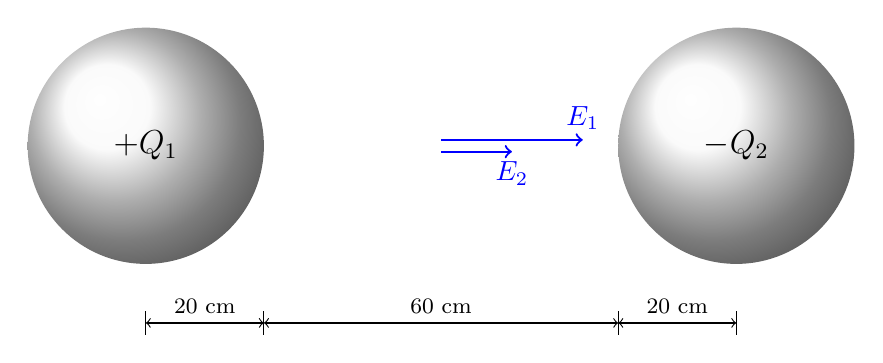
\begin{tikzpicture}[scale=0.75]
		\shade [ball color = gray!5] (-5,0) circle (2) node {{\large $+Q_1$}};
		\shade [ball color = gray!5] (5,0) circle (2) node {{\large $-Q_2$}};;
		\draw[thick,blue,->] (0,0.1) -- (2.4,0.1) node[above]{$E_1$};
		\draw[thick,blue,->] (0,-0.1) -- (1.2,-0.1) node[below]{$E_2$};
		\draw[<->] (-5,-3) -- (-3,-3) node[midway,above]{{\footnotesize 20 cm}};
		\draw[<->] (-3,-3) -- (3,-3) node[midway,above]{{\footnotesize 60 cm}};
		\draw[<->] (5,-3) -- (3,-3) node[midway,above]{{\footnotesize 20 cm}};
		\foreach \gang in {-5,-3,3,5} \draw (\gang,-2.8) --++ (0,-0.4);
	\end{tikzpicture}
\end{figure}
	
\sol field strengths due to the two spheres are in same direction
\begin{equation*}
E = E_1 + E_2 = \frac{1}{\ec}\left( \frac{Q_1}{r_1^2} + \frac{Q_2}{r_2^2} \right) = 8.99 \times 10^9 \times \left( \frac{2.0\times 10^{-6}}{0.25^2} + \frac{1.0\times 10^{-6}}{0.25^2}\right) \approx 4.32\times 10^5 \NpC
\end{equation*}

field strength points to the right

force on dust particle: $F = Eq = 4.32\times 10^5 \times 1.4\times10^{-8} \approx 5.6\times10^{-3} \text{ N}$

dust particle is negatively-charged means force is opposite to field strength

so force on dust particle acts to the left \eoe

\question{When the charge on the Van de Graaff generator is $4.0\times10^{-7} \text{ C}$, the electric field strength at the sphere's surface is $2.4 \times 10^6 \Vpm$. Determine the additional charge added to the sphere if the field strength at the surface becomes $3.0 \times 10^6 \Vpm$.}

\question{Two positively charged particles $A$ and $B$ are situated in a vacuum. Point P lies on the line joining the centres of the two spheres and is a distance $x$ from $A$. Sketch the variation with $x$ of electric field strength $E$ due to the two particles.}

\subsubsection{electric field lines}
we can use \keypoint{electric field lines} to visualize an electric field\index{field line!electric field line}

\cmt \emph{arrows} of field lines show direction of the field

field lines always tend to leave positive charge, and end up at negative charges

\cmt \emph{density} or spacing of lines show strength of the field

\example{Sketch the electric field around a positively-charged sphere or a negatively charged sphere, and explain why they can be considered as point charges.}\label{ex-radial-efield}
	
\begin{center}
	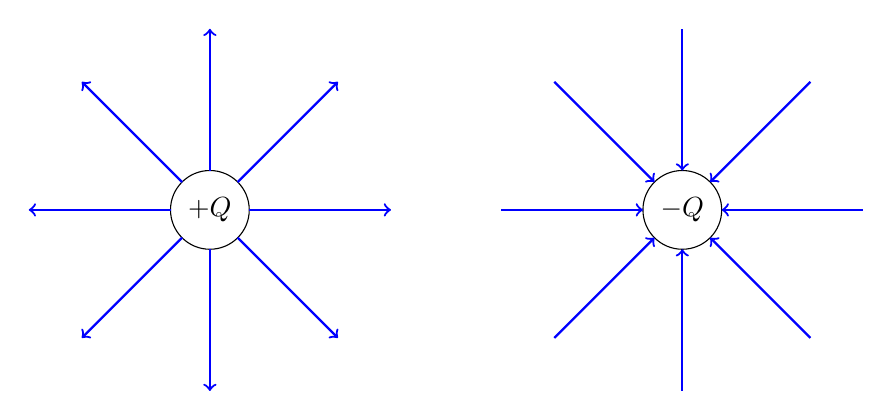
\begin{tikzpicture}[scale=1]
			\draw (-3,0) node{$+Q$} circle [radius=0.5];
			\foreach \s in {0,45,90,...,315}
			\draw [blue, thick, ->] (-3,0) ++ (\s:0.5) -- ++(\s:1.8);

			\draw (3,0) node{$-Q$} circle [radius=0.5];
			\foreach \s in {0,45,90,...,315}
			\draw [blue, thick, <-] (3,0) ++ (\s:0.5) -- ++(\s:1.8);
	\end{tikzpicture}
\end{center}

\vspace*{-6pt} field lines of either case are \emph{radial}, i.e., perpendicular to surface

field lines appear to start from or converge towards centre of the sphere

so charged spheres act like point charges \eoe



\example{Field lines between two oppositely-charged large metal plates.}

\begin{center}
	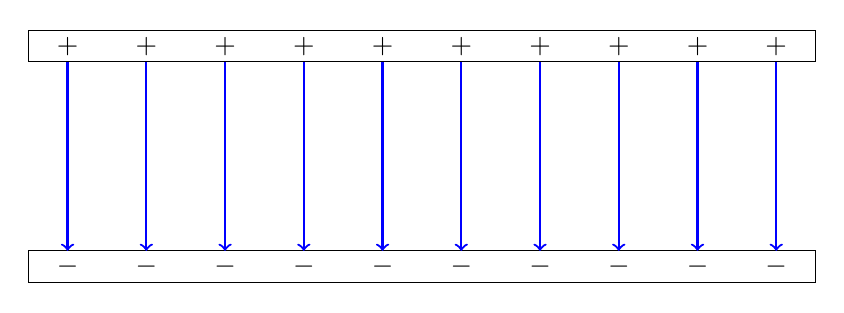
\begin{tikzpicture}
		\draw (-5,1.2) rectangle (5,1.6);
		\draw (-5,-1.2) rectangle (5,-1.6);
		\foreach \charge in {-4.5,-3.5,...,4.5}{
			\draw (\charge,1.4) node {$+$} (\charge,-1.4) node {$-$};
			\draw[thick,blue,->] (\charge,1.2) --++ (0,-2.4);	
		}
	\end{tikzpicture}
\end{center}

\vspace*{-6pt} field lines are \emph{parallel} and equally spaced, so this is a \emph{uniform} electric field \eoe

\example{Field pattern due to two charges of equal magnitude.}

\begin{center}
	\noindent\begin{minipage}{0.48\textwidth}
		\begin{center}
			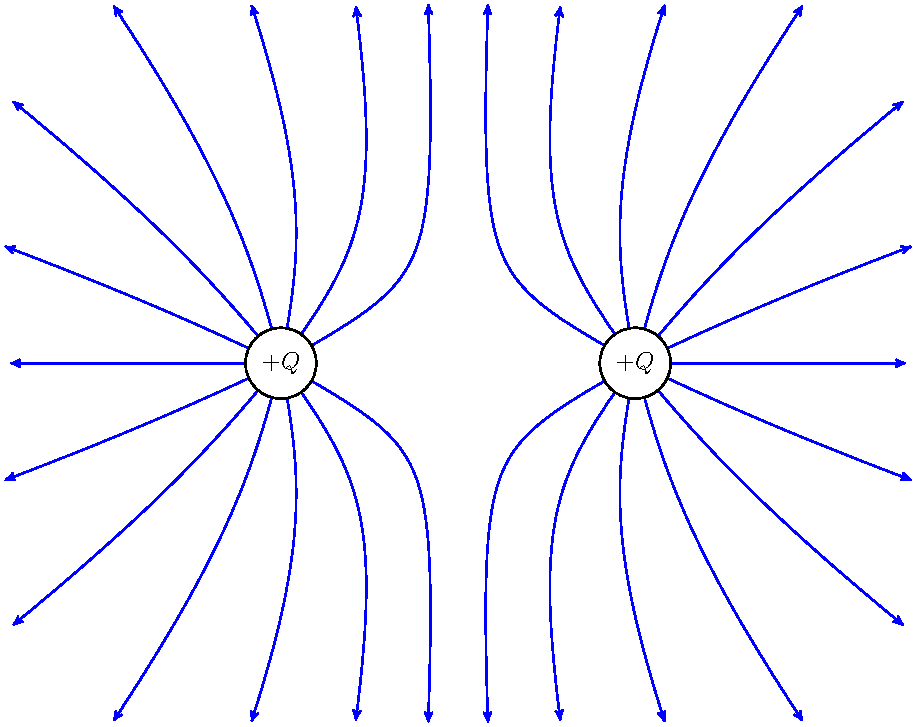
\includegraphics[width=7.2cm]{f-lines-eq-ch.pdf}
			\begin{equation*}
			\text{two positive charges}
			\end{equation*}
		\end{center}
	\end{minipage}\hfill
	\begin{minipage}{0.48\textwidth}
		\begin{center}
			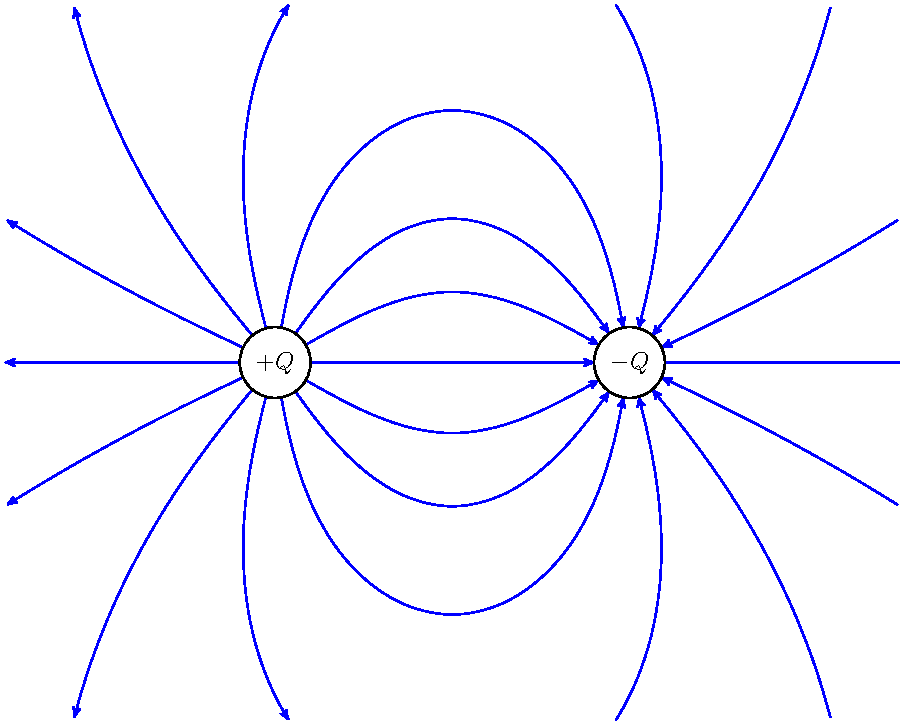
\includegraphics[width=7.2cm]{f-lines-op-ch.pdf}
			\begin{equation*}
			\text{two opposite charges} \teoe
			\end{equation*}
		\end{center}	
	\end{minipage}
\end{center}




\subsection{potential \& potential energy }

\subsubsection{electric potential energy}
\label{sec:electric-potential}

gain/loss in \keypoint{electric potential energy}\index{electric field!electric potential energy} is defined as work done against/by electric force

(compare everything in this section with what you have learned about gravitational P.E.!)

let's start to derive the electrical P.E. between two charges $Q$ and $q$ separated by $r$

again we define $E_p=0$ at $r=\infty$ (choice of zero potential energy, no force so no P.E.), then

\begin{ilight}
	\keypoint{electric potential energy} is equal to the work done by electric force to bring a charge to a specific position from \emph{infinity}
\end{ilight} 

moving a test charge $q$ from $r=\infty$ to a distance of $r$ from $Q$

\begin{center}
\begin{tikzpicture}[scale=0.8]
\draw [fill] (-4,0) circle [radius=0.1];
\node[below] at (-4,-0.1) {$Q$};
\draw [fill] (8,0) circle [radius=0.1];
\node[below] at (8,-0.1) {$q$};
\draw [thick, <->] (0,-1.2) --(-4,-1.2) node[above,midway]{$r$};
\draw [thick,dashed,gray,->] (7.7,0) -- (0.3,0) node[above,midway]{\textcolor{black}{$W$}};
\draw [fill] (0,0) circle [radius=0.1];
\draw (8,-1) node{$\infty$};
\end{tikzpicture}
\end{center}

work done by electric force: $W=\int^r_\infty F dr = \int^r_\infty \frac{Qq}{\ec} \frac{\dd x}{x^2} = - \frac{Qq}{\ec x}\bigg|^r_\infty = - \frac{Qq}{\ec r} $

\eqyskip

since $\Delta E_p=-W$, we find: $E_p(r) - E_p(_\infty) = \frac{Qq}{\ec r}$

but $E_p(_\infty) = 0$,  so electric P.E. between two charges $Q$ and $q$ is $\boxed{E_p(r) = \frac{Qq}{\ec r}}$

\cmt as $r \to \infty$, $E_p \to 0$, this agrees with our definition for zero P.E. point

\cmt for like charges, $Qq > 0$, so $E_p > 0$

to bring like charges closer, work must be done to overcome their \emph{repulsion}, P.E. increases

minimum P.E. $E_p(\infty)=0$ at infinity, so positive P.E. at finite $r$

\cmt for opposite charges, $Qq < 0$, so $E_p < 0$

to pull opposite charges apart, work must be done to overcome their \emph{attraction}, P.E. increases

maximum P.E. $E_p(\infty)=0$ at infinity, so negative P.E. at finite $r$

\cmt electric P.E. is a \emph{scalar quantity}, sign is important

repulsion implies positive P.E., and attraction implies negative P.E.

sign of P.E. is hidden in polarities of charges


\example{In $\alpha$-particle scattering experiment, we fire $\alpha$-particles ($_2^4\alpha$) towards a thin gold ($_{\phantom{0}79}^{197}\text{Au}$) foil in hope of gaining information about the nucleus. The size of a typical nucleus is about $10^{-14}$m, what is the minimum initial speed for $\alpha$-particles so that radius of gold nucleus can be determined?}
	
\sol as $\alpha$-particle approaches the nucleus, it slows down due to the repulsive interaction

kinetic energy decreases and electric potential energy increases

if it gets close enough to the nucleus before coming to a stop, nuclear radius can be estimated

{

\centering

$\text{K.E. loss} = \text{P.E. gain} \RA \frac{1}{2}mu^2 - \underbrace{\frac{1}{2}mv^2}_0 = E_p(r) - \underbrace{E_p(\infty)}_0 \RA  \frac{1}{2}mu^2= \frac{Qq}{4\pi\epsilon_0r}$

}

\begin{equation*}
	\frac{1}{2}\times4\times1.66\times10^{-27}\times u^2 = \frac{79\times1.60\times10^{-19}\times2\times1.60\times10^{-19}}{4\pi\times8.85\times10^{-12}\times10^{-14}} \RA
	u\approx 3.3\times10^7\mps \teoe
\end{equation*}

\question{A metal sphere of radius 20 cm carries a charge of $5.0\times10^{-7}$ C. A proton is sent towards the sphere at a speed of $1.8\times10^6 \mps$. Can the proton reach the surface of the sphere?}



\subsubsection{electric potential}

it is also useful to define the \emph{electric potential} for any specific point in a field

electric potential can be thought as the electric potential energy per unit charge: $V = \frac{E_p}{q}$

\begin{ilight}
	\keypoint{electric potential}\index{electric field!electric potential} is the work needed to bring a unit positive charge from infinity
\end{ilight}

\cmt unit: $[V] = \text{ J C}^{-1} = \text{V}$

\cmt electric potential due to an isolated source $Q$: $V = \frac{E_p}{q} = \frac{\frac{Qq}{\ec r}}{q} \RA \boxed{V = \frac{Q}{4\pi\epsilon_0 r}}$

\cmt potential at infinity vanishes: $V_\infty = 0$

\cmt electric potential can take both signs

the sign depends on whether unit positive charge is repelled or attracted by the source

for positively-charged sources $V>0$, while for negatively-charged sources $V<0$

\cmt electric potential is a \emph{scalar} quantity

to find combined potential due to multiple charges, add up contributions of each charge

\example{An electron is accelerated from rest through a potential difference of 600 V.
	
Find the final speed of the electron.}

\sol gain in K.E. = change in electric P.E. $\RA \frac{1}{2}mv^2 = q\Delta V$
\eqyskip\begin{equation*}
	v = \sqrt{\frac{2q\Delta V}{m}} = \sqrt{\frac{2\time 1.60\times10^{-19}\times600}{9.11\times10^{-31}}} \approx 1.45\times10^7 \mps \teoe
\end{equation*}

\example{Two small metal spheres $A$ and $B$ are in a vacuum. Sphere $A$ has charge $+20$ pC and sphere $B$ has charge $+84$ pC. The arrangement is shown below.}

\begin{figure}[ht]
	\centering
	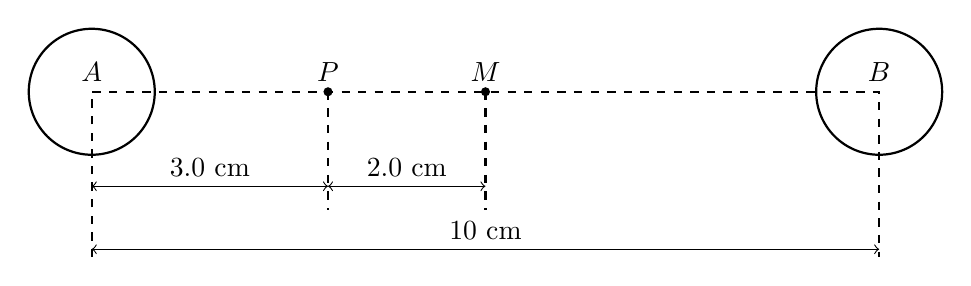
\begin{tikzpicture}
		\draw[thick] (-5,0) circle(0.8) node[above]{$A$} (5,0) circle(0.8) node[above]{$B$};
		\draw[thick,dashed] (-5,-2.1) -- (-5,0) -- (5,0) -- (5,-2.1) (-2,0) node[above]{$P$} -- (-2,-1.5)
		(0,0) node[above]{$M$} -- (0,-1.5);
		\draw[fill] (-2,0) circle(0.05);
		\draw[fill] (0,0) circle(0.05);
		\draw[<->] (-5,-2.0) -- (5,-2.0) node[midway,above]{$10$ cm};
		\draw[<->] (-5,-1.2) -- (-2,-1.2) node[midway,above]{$3.0$ cm};
		\draw[<->] (0,-1.2) -- (-2,-1.2) node[midway,above]{$2.0$ cm};
	\end{tikzpicture}
\end{figure}

(a) Find the electric potential at point $P$ and point $M$ respectively.

(b) Find the work done to move an $\alpha$-particle from $P$ to $M$.

\sol combined electric potential: $V = V_A + V_B = \frac{1}{\ec}\left(\frac{Q_A}{r_A} + \frac{Q_B}{r_B} \right)$

\eqyskip

at $P$: $V_P = 8.99\times10^9 \times \left( \frac{+20 \times 10^{-12}}{0.030} + \frac{+84 \times 10^{-12}}{0.070} \right) \approx 16.8 \text{ V}$

\eqyskip

at $M$: $V_M = 8.99\times10^9 \times \left( \frac{+20 \times 10^{-12}}{0.050} + \frac{+84 \times 10^{-12}}{0.050} \right) \approx 18.7 \text{ V}$

from $P$ to $M$: $W = \Delta E_p = q\Delta V = q(V_M- V_P) = 2\times1.60\times10^{-19}\times(18.7-16.8) \approx 6.2\times10^{-19} \text{ J}$ \eoe

\example{$A$ and $B$ are two positively-charged spheres of radius 1.0 cm. A proton $P$ initially at rest on the surface of $A$ moves along the line joining the centres of the two spheres. The variation with distance $x$ from the centre of $A$ of electric potential $V$ at point $P$ is given.}\label{ex-V-of-two-pcs}

\begin{figure}[ht]
	\centering
	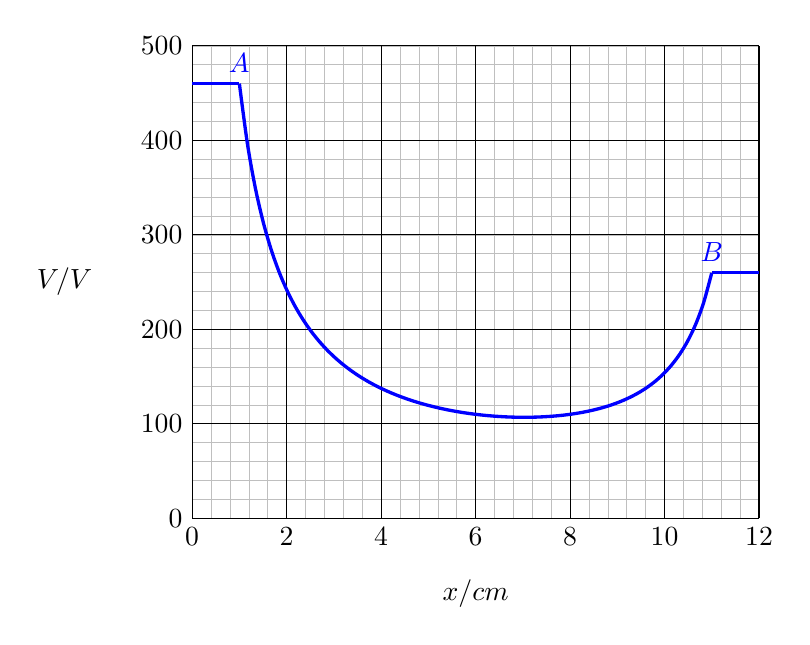
\begin{tikzpicture}[scale=1.2]
		\draw[style=help lines,step=0.2,gray!50] (0,-0) grid (6,5);
		\draw[step=1] (0,0) grid (6,5);
		\draw [very thick, color=blue, domain=0.5:5.5, smooth, samples=60, variable=\x] plot (\x,{2.2/\x + 1.1/(6-\x)});
		\draw[very thick,blue] (0,4.6) --++ (0.5,0) node[above]{$A$};
		\draw[very thick,blue] (5.5,2.6) node[above]{$B$} --++ (0.5,0);
		\foreach \x in {0,100,200,300,400,500} \node[left] at (0,\x/100) {$\x$};
		\foreach \x in {0,2,4,6,8,10,12} \node[below] at (\x/2,0) {$\x$};
		\node at (-1.35,2.5) {$V/\text{V}$};
		\node at (3,-0.8) {$x/\text{cm}$};
	\end{tikzpicture}
\end{figure}

\rcyskip (a) Find the maximum speed as the proton moves from $A$ to $B$.

(b) Find the speed when the proton reaches surface of $B$.

\sol increase in K.E. = loss in P.E., so: $\frac{1}{2}mv^2 - 0 = q\Delta V \RA \frac{1}{2}mv^2 = q(V_A - V_P)$

maximum speed when $\Delta V$ is maximum, or $V_P = 107 \text{ V}$ becomes minimum (at $x = 7.2$ cm)
\begin{equation*}
	\frac{1}{2}\times1.67\times10^{-27}\times v^2_\tmax = 1.60\times10^{-19} \times (460-107) \RA v_\tmax \approx 2.60\times10^5 \mps
\end{equation*}

at surface of $B$, $V_P = 260 \text{ V}$ (at $x=11.0$ cm)
\begin{equation*}
\frac{1}{2}\times1.67\times10^{-27}\times v^2_B = 1.60\times10^{-19} \times (460-260) \RA v_B \approx 1.96\times10^5 \mps \teoe
\end{equation*}

\question{Electrical breakdown occurs when electric field strength at surface of a metal sphere exceeds $5.0 \times 10^6 \NpC$. Given that the radius of the sphere is 16 cm. What is the electric potential at the surface when electrical breakdown occurs?}

\question{Two charged particles $A$ and $B$ are separated by 20 cm. $P$ is a point on the line $AB$. Given that particle $A$ carries charge $+7.2 \text{ }\mu\text{C}$, and electric potential is zero where $AP = 5.0$ cm. Find the electric charge of $B$.}

\question{A particle with specific charge (ratio of its electric charge to its mass) $+9.58\times10^7 \text{ C kg}^{-1}$ is moving towards a fixed metal sphere. The sphere has a potential of $+500$ V. The initial speed of the particle is $3.0\times10^5 \mps$ when it is a large distance from the sphere. Determine whether the particle can reach the surface of the sphere.}


\subsubsection{equipotential lines}

to show potential distributions, we draw \keypoint{equipotential lines}\index{equipotential lines}
\footnote{In three dimensions, these lines form equipotential \emph{surfaces}.}

points on same equipotential line have constant electric potential

i.e., equipotential lines are \emph{contour lines} of equal electric potential

\cmt for a field near a point charge, equipotential lines are a set of \emph{concentric} circles

\begin{center}
	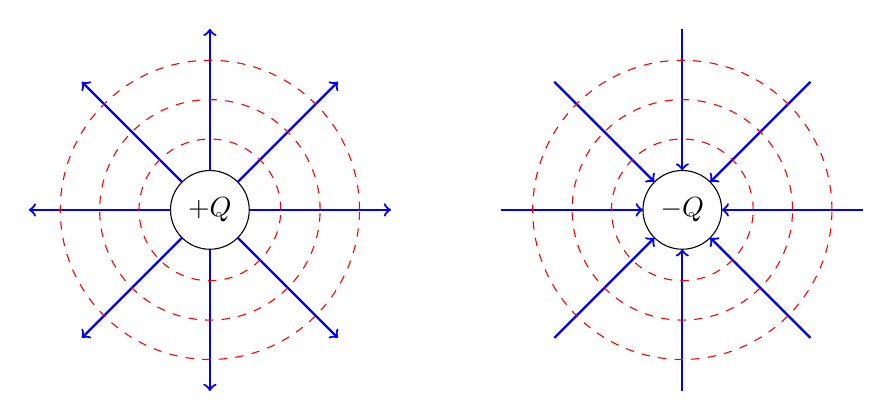
\begin{tikzpicture}[scale=1]
	\draw (-3,0) node{$+Q$} circle [radius=0.5];
	\foreach \s in {0,45,90,...,315}
	\draw [blue, thick, ->] (-3,0) ++ (\s:0.5) -- ++(\s:1.8);
	
	\draw (3,0) node{$-Q$} circle [radius=0.5];
	\foreach \s in {0,45,90,...,315}
	\draw [blue, thick, <-] (3,0) ++ (\s:0.5) -- ++(\s:1.8);
	
	\foreach \s in {0.9,1.4,1.9}{
		\draw [red,dashed] (-3,0) circle(\s) (3,0) circle(\s);}
	\end{tikzpicture}
\end{center}

\cmt for uniform fields, equipotential lines are a set of \emph{parallel} straight lines

\begin{center}
	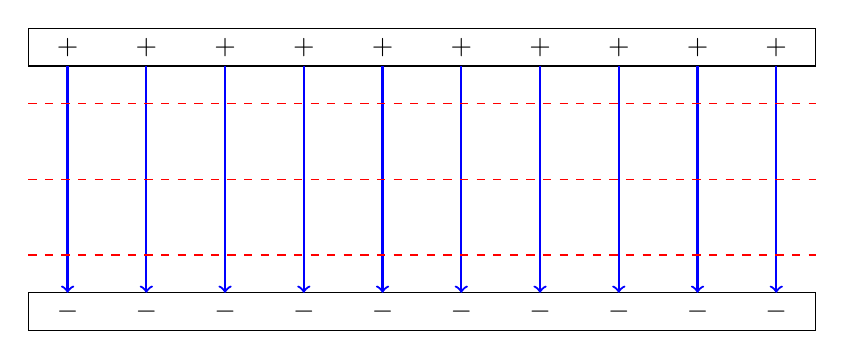
\begin{tikzpicture}[yscale=1.2]
	\draw (-5,1.2) rectangle (5,1.6);
	\draw (-5,-1.2) rectangle (5,-1.6);
	\foreach \charge in {-4.5,-3.5,...,4.5}{
		\draw (\charge,1.4) node {$+$} (\charge,-1.4) node {$-$};
		\draw[thick,blue,->] (\charge,1.2) --++ (0,-2.4);	
	}
	\foreach \s in {-0.8,0,0.8} \draw[red,dashed] (-5,\s) -- (5,\s);
	\end{tikzpicture}
\end{center}
	

	
\cmt equipotential lines are always perpendicular to the electric field lines
	
moving along an equipotential line requires no work done

\example{Field lines and equipotential lines due to two charges of various magnitudes}

\begin{center}
	\noindent\begin{minipage}{0.48\textwidth}
		\begin{center}
			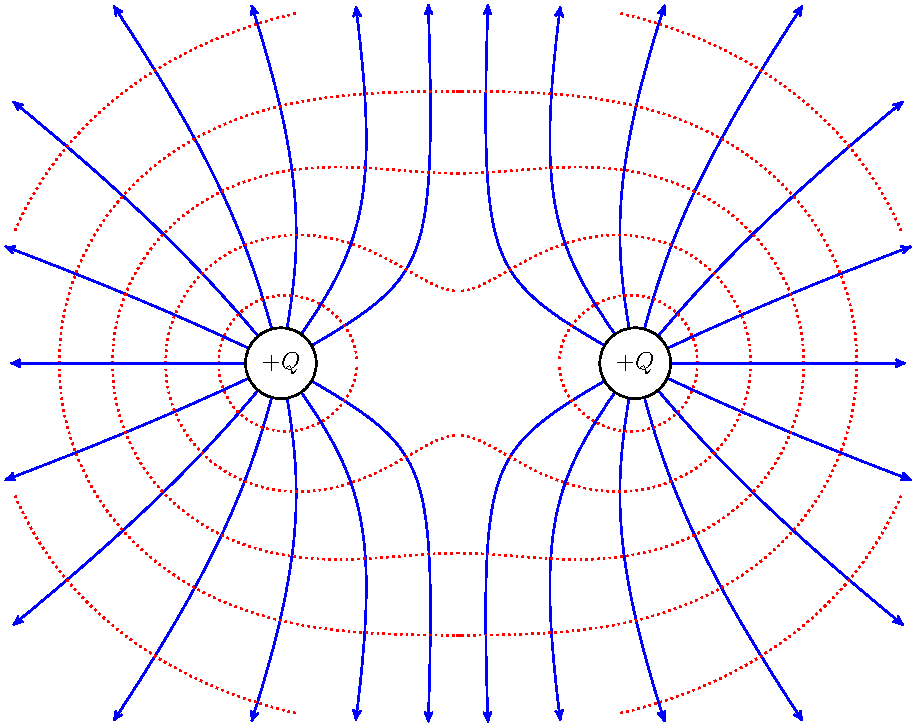
\includegraphics[width=7cm]{f-all-eq-ch.pdf}
		\end{center}
	\end{minipage}\hfill
	\begin{minipage}{0.48\textwidth}
		\begin{center}
			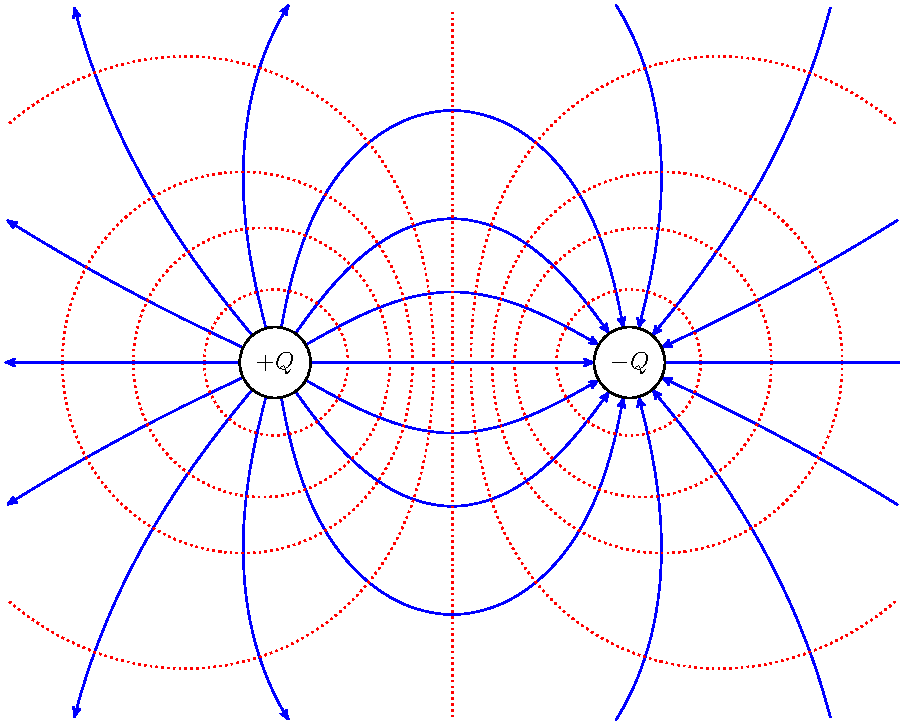
\includegraphics[width=7cm]{f-all-op-ch.pdf}
		\end{center}
	\end{minipage}
\end{center}

\begin{center}	
	\noindent\begin{minipage}{0.48\textwidth}
		\begin{center}	
			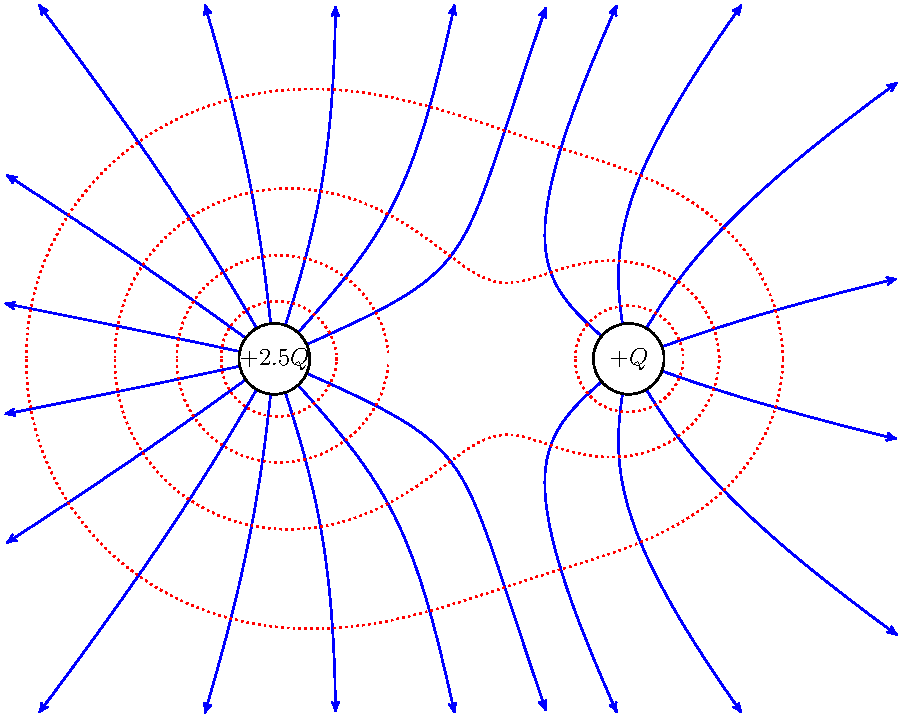
\includegraphics[width=7cm]{Q2p.pdf}
			\end{center}
		\end{minipage}\hfill
	\begin{minipage}{0.48\textwidth}
		\begin{center}
			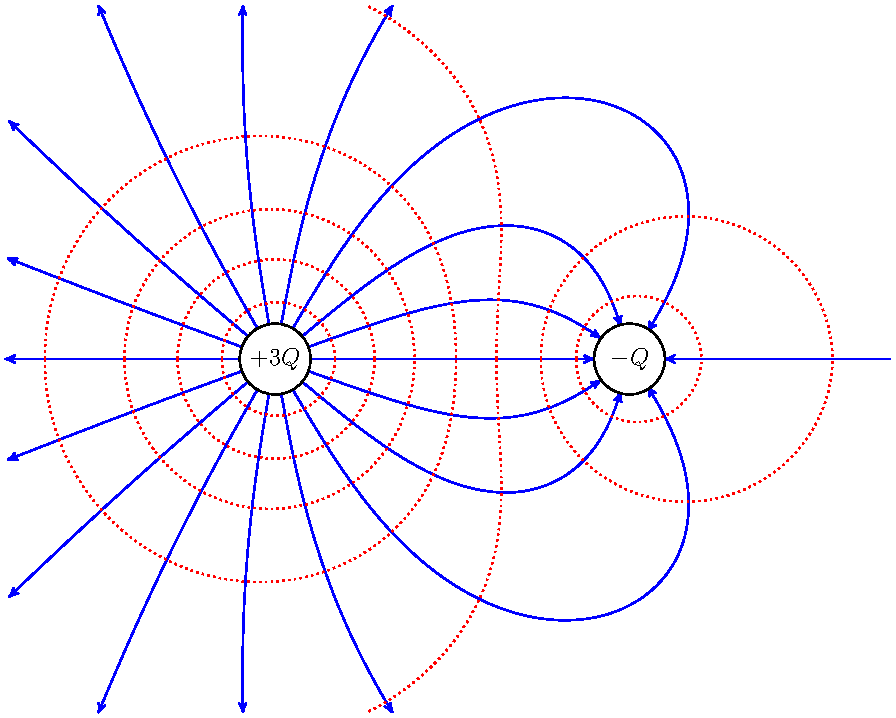
\includegraphics[width=7cm]{Q4n.pdf}
		\end{center}
	\end{minipage}
\end{center}

\begin{center}	
	\noindent\begin{minipage}{0.48\textwidth}	
		\begin{center}	
			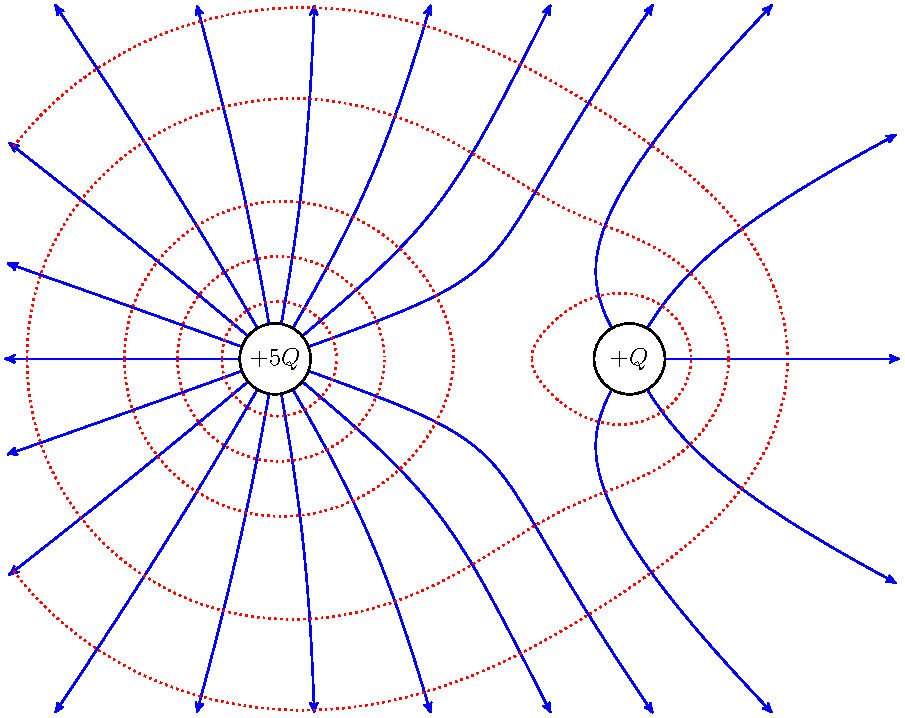
\includegraphics[width=7cm]{Q5p.pdf}
		\end{center}
	\end{minipage}\hfill
	\begin{minipage}{0.48\textwidth}
		\begin{center}
			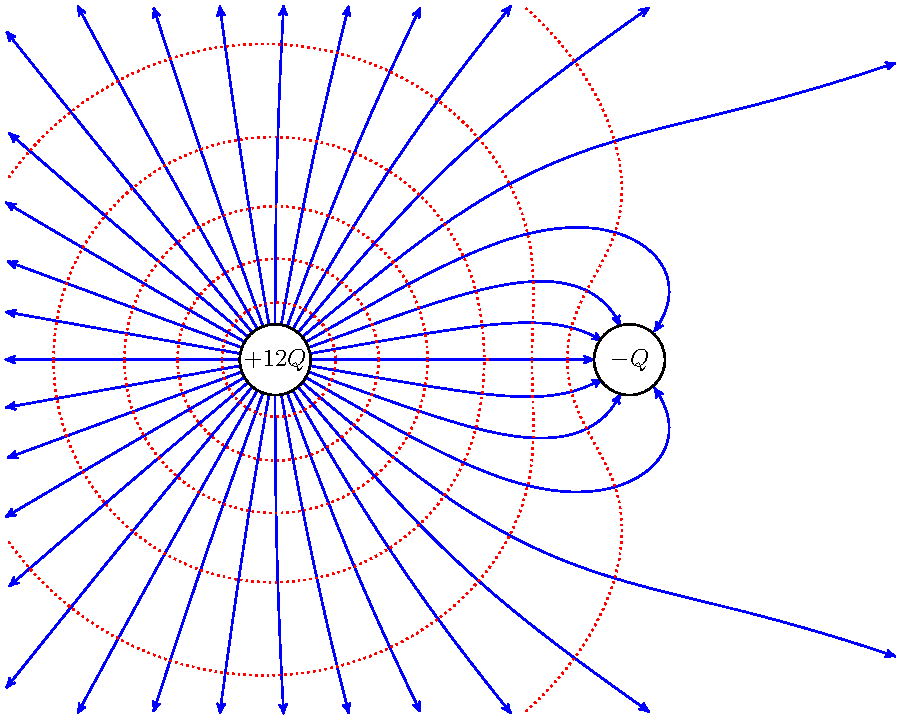
\includegraphics[width=7cm]{Q12n.pdf}
		\end{center}	
	\end{minipage}
\end{center}



\subsection{further discussions on electric fields}

\subsubsection{comparison with gravitational fields}

both gravitational and electric force are described by inverse square law, so it follows that the mathematical language for both theories are very similar

\cmt physical quantities that describe gravitational/electric fields

\begin{center}
	\begin{tabular}{|c|c|c|}
		\hline
		& vector description & scalar description \\ \hline 
		interaction between two masses/charges & force $F$ & potential energy $E_p$ \\ \hline
		effect of source mass/charge & field $g$/$E$ & potential $\varphi$/$V$ \\ \hline
	\end{tabular}
\end{center}

\cmt comparing gravitational field with electric field
\footnote{Note that there is no negative mass, gravitational force always interacts attractively. This is the fundamental difference between gravitational fields and electric fields.}

\begin{center}
{\renewcommand{\arraystretch}{1.28}
\begin{tabular}{|c|c|c|c|}
\hline
& gravitational field & electric field & meaning \\ \hline 
force & $F=(-)G \frac{Mm}{r^2}$ & $F=\frac{1}{4\pi\epsilon_0} \frac{Qq}{r^2}$ & force between masses/charges\\ [1ex] \hline
field strength & $g= \frac{F}{m} = (-)G \frac{M}{r^2}$ & $E= \frac{F}{q} = \frac{1}{4\pi\epsilon_0} \frac{Q}{r^2}$ & force per unit mass/charge\\ [1ex] \hline
potential energy &  $E_p = -G \frac{Mm}{r}$ & $E_p=\frac{1}{4\pi\epsilon_0} \frac{Qq}{r}$ & related to work done by force \\ [1ex] \hline
potential & $\varphi = \frac{E_p}{m} = -G \frac{M}{r}$ & $V = \frac{E_p}{q} = \frac{1}{4\pi\epsilon_0} \frac{Q}{r}$ & energy per unit mass/charge\\ [1ex] \hline
\end{tabular}}
\end{center}

\cmt similarities between gravitational field and electric field

\begin{itemize}
	\item[-] force and field strength both obey \emph{inverse square laws}
	
	\item[-] potential energy and potential is inversely proportional to separation
	
	\item[-] no potential energy and no potential at infinite separation
\end{itemize}

\cmt differences between gravitational field and electric field

mass (source of gravity) is always positive, but electric charges can be positive or negative

this fact leads to many fundamental differences between the two force fields

\begin{itemize}
\item[-] electric force can be repulsive or attractive, but gravitational force is always attractive

\item[-] electric potential can take both signs, but gravitational potential is always negative
\end{itemize}

\subsubsection{electric field inside conductors}\label{inside-conductors}

consider electric field \emph{inside} a metal conductor carrying charge $Q$

conductor means there are free charge carriers that can move around 

but charge distribution should be stable for a charged conductor (no circulating currents)

so charge carriers must experience no force, i.e., field strength inside conductor is zero

put it the other way round, if there is an excess field, it will push free charge carriers to move around, until they are distributed so that the field inside the conductor becomes zero

moreover, there shall be no potential difference between any two points inside the conductor, otherwise charge carriers would flow, so electric potential must be constant

\begin{ilight}
	\centering
	
	electric field strength is everywhere zero inside a conductor: $E=0$
	
	electric potential is everywhere constant inside a conductor: $V=\text{const}$
\end{ilight}

\example{Consider the electric field due to a metal sphere of radius $R$ carrying charge $Q$. Plot the variation with the distance $r$ from sphere's centre of the field strength, and the variation with $r$ of the electric potential.}\label{ex-metal-sphere}


\sol charge $Q$ is uniformly spread out on \emph{surface} of sphere

viewed from \emph{outside}, the sphere appears to have all of its charge concentrated at the centre

so it can be modelled as a point charge due to its symmetric distribution of charges

electric field strength at distance $r$ from sphere's centre is: $E = \frac{Q}{\ec r^2}$ for $r>R$

electric potential at distance $r$ from sphere's centre is: $V=\frac{Q}{4\pi\epsilon_0r}$ for $r>R$

\emph{inside} the sphere, i.e., for $r<R$, we have $E=0$, and $V=\frac{Q}{\ec R} = \text{const}$ \eoe

\begin{figure}[ht]
	\centering
	\noindent\begin{minipage}{0.45\linewidth}
		\centering
		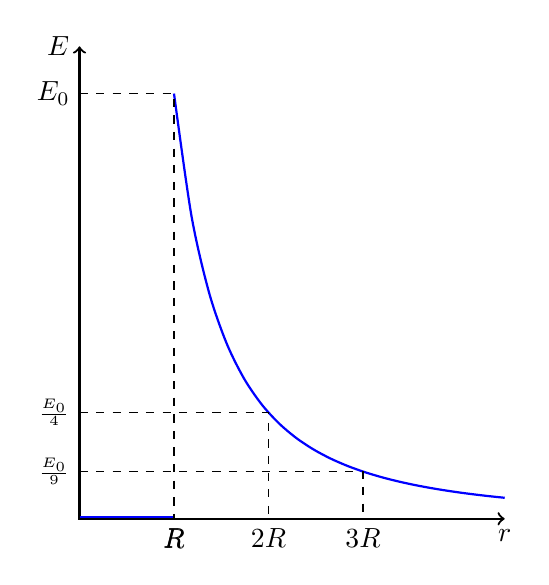
\begin{tikzpicture}[yscale=1.2,xscale=1.2]
		\draw[thick,<->] (0,5) node[left]{$E$} -- (0,0) -- (1,0) node[below]{$R$} -- (4.5,0) node[below]{$r$};
		\draw [thick,color=blue,domain=1:4.5,samples=20,smooth,variable=\x] plot (\x,{4.5/\x/\x});
		\draw[thick,blue] (0,0.02) -- (1,0.02);
		\draw[dashed] (0,4.5) node[left]{$E_0$} -- (1,4.5) -- (1,0) node[below]{$R$};
		\draw[dashed] (0,4.5/4) node[left]{{\scriptsize $\frac{E_0}{4}$}} -- (2,4.5/4) -- (2,0) node[below]{$2R$};
		\draw[dashed] (0,4.5/9) node[left]{{\scriptsize $\frac{E_0}{9}$}} -- (3,4.5/9) -- (3,0) node[below]{$3R$};
		\end{tikzpicture}
		

	\end{minipage}
	\begin{minipage}{0.45\linewidth}
		\centering
		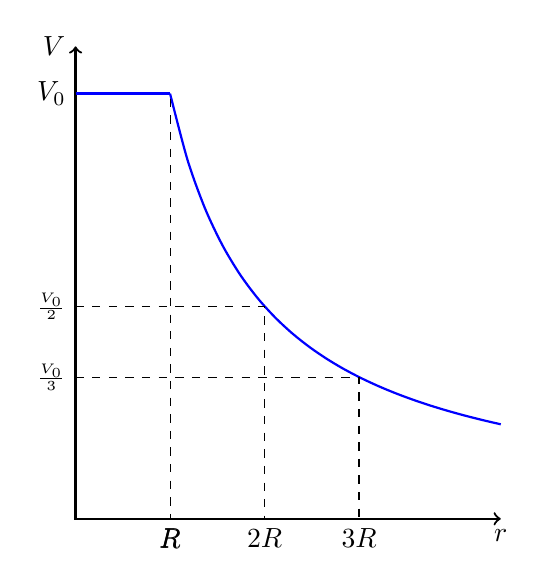
\begin{tikzpicture}[yscale=1.2,xscale=1.2]
		\draw[thick,<->] (0,5) node[left]{$V$} -- (0,0) -- (1,0) node[below]{$R$} -- (4.5,0) node[below]{$r$};
		\draw [thick,color=blue,domain=1:4.5,samples=20,smooth,variable=\x] plot (\x,{4.5/\x});
		\draw[dashed] (0,4.5) node[left]{$V_0$} -- (1,4.5) -- (1,0) node[below]{$R$};
		\draw[dashed] (0,4.5/2) node[left]{{\scriptsize $\frac{V_0}{2}$}} -- (2,4.5/2) -- (2,0) node[below]{$2R$};
		\draw[dashed] (0,4.5/3) node[left]{{\scriptsize $\frac{V_0}{3}$}} -- (3,4.5/3) -- (3,0) node[below]{$3R$};
		\draw[thick,blue] (0,4.5) -- (1,4.5);
		\end{tikzpicture}
		

	\end{minipage}
\captionsetup{labelformat=empty}

\caption{Example \ref{ex-metal-sphere}: field strength and potential due to a charged metal sphere}
\end{figure}


\question{State whether the two spheres in Example \ref{ex-V-of-two-pcs} are conductors. State what feature of the potential graph supports your answer.}

\question{You might have the experience that your mobile phone signal gets much weaker when you get into an elevator. Explain why this happens.}

\subsubsection{field strength \& potential}\label{field-strength-potential}

for a small displacement $\Delta r$ in an electric field, change in potential $\Delta V$ is

{

\centering

$\Delta V = \frac{\Delta E_p}{q} \xlongequal{\Delta E_p=-W} - \frac{\Delta W}{q} = - \frac{F \Delta r}{q} \xlongequal{F=Eq} - E \Delta r \RA E = - \frac{\Delta V}{\Delta r}$

}

\eqyskip as change in displacement $\Delta r \to 0$, we have $\boxed{E = - \frac{\dd V}{\dd r}}$

therefore we have the following theorem:

\begin{ilight}
	\centering field strength is negative gradient of potential with respect to displacement
\end{ilight}

can also consider change in potential $\Delta V$ for large distance due to work done in a field

{
	
\centering

$\Delta V= \int \dd V \xlongequal{E = -\dd V/\dd r}  \int (-)E \dd r =  -\int E \dd r$
\footnote{The expression is implicitly integrated from initial position to final position.}

}

\eqyskip this gives the inverse relation: $\boxed{\Delta V = -\int E \dd r}$
\footnote{These equations are correct if the charge is moving in the parallel direction to the field, i.e., the motion is along the field lines. But an object can move in all directions in the field. More rigorously, if we take the vector nature of electric field into account, we should write $\Delta V = - \int \mathbf{E}\cdot\dd\mathbf{r}$, and $\mathbf{E} = - \frac{\partial V}{\partial \mathbf{r}}$. ($\star$)}

\cmt given a $V$-$r$ graph, gradient of curve gives field strength

conversely, given a $E$-$r$ graph, area under curve gives change in potential

\cmt can also write $F = - \frac{\dd U}{\dd r}$ and $\Delta U = -\int F \dd r$

force always acts in a direction to lower the potential energy of an object
\footnote{This result can be generalised to a very important principle of physical laws called the \emph{least action principle}. It states that any motion of a system tends to minimise the action, a physical quantity related to the energy of the system. This fundamental law plays a crucial role in the study of theoretical physics. ($\star$)}

\example{The variation of electric potential near a charged object is shown on the graph. Calculate the electric field strength at 5.0 cm from the centre of the object.}\label{ex-grad-pot}

\begin{figure}[ht]
	\centering
	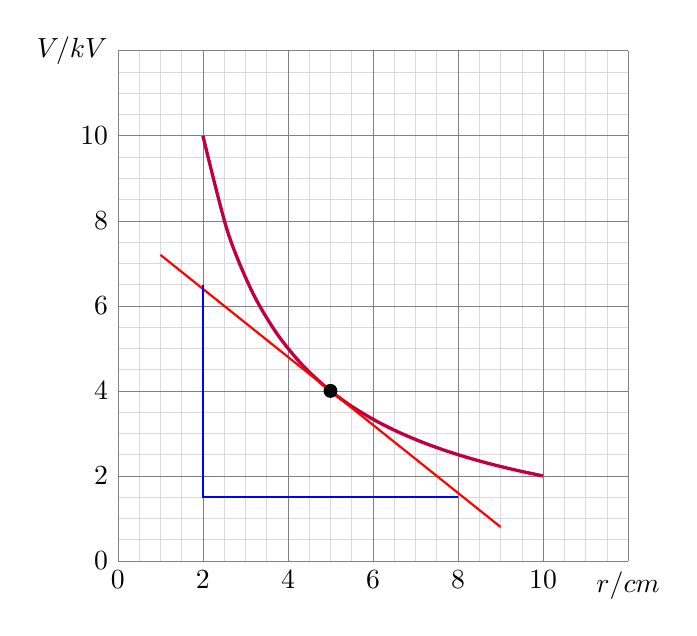
\begin{tikzpicture}[scale=0.54]
	\draw[style=help lines,step=0.5,gray!30] (0,0) grid (12,12);
	\draw[style=help lines,step=2] (0,0) grid (12,12);
	\draw [thick] (12,0) node[below]{$r/\text{cm}$};
	\draw [thick] (0,12) node[left]{$V/\text{kV}$};
	\foreach \s in {0,2,...,10}
	{
		\draw (\s,0) node[below]{\s};
		\draw (0,\s) node[left]{\s};
	}
	\draw[very thick,purple,domain=2:10,samples=15,smooth,variable=\x] plot (\x,20/\x);
	\draw[thick,red,domain=1:9,samples=2,smooth,variable=\x] plot (\x,-0.8*\x+8);
	\draw[fill] (5,4) circle[radius=0.15];
	\draw[thick,blue] (2,6.5) -- (2,1.5) -- (8,1.5);
	\end{tikzpicture}
\end{figure}

\sol draw tangent to the graph at $r=5.0\text{ cm}$ (red line), gradient of tangent gives field strength:

$ \text{gradient} = \frac{\Delta V}{\Delta r} = \frac{(1.5-6.5)\times 10^3}{(8.0-2.0)\times10^{-2}} \approx  -8.3\times10^4 \Vpm \RA E = -\frac{\Delta V}{\Delta r} = 8.3\times10^4 \Vpm $ \eoe 

\question{Show that the charged object in Example \ref{ex-grad-pot} behaves like a point charge. Determine the charge it carries, and hence calculate the field strength at $r=5.0$ cm.}

\example{The variation of electrical potential along a certain line is shown. State and explain where in the field an electron will experience the greatest force.}

\begin{figure}[ht]
	\centering
	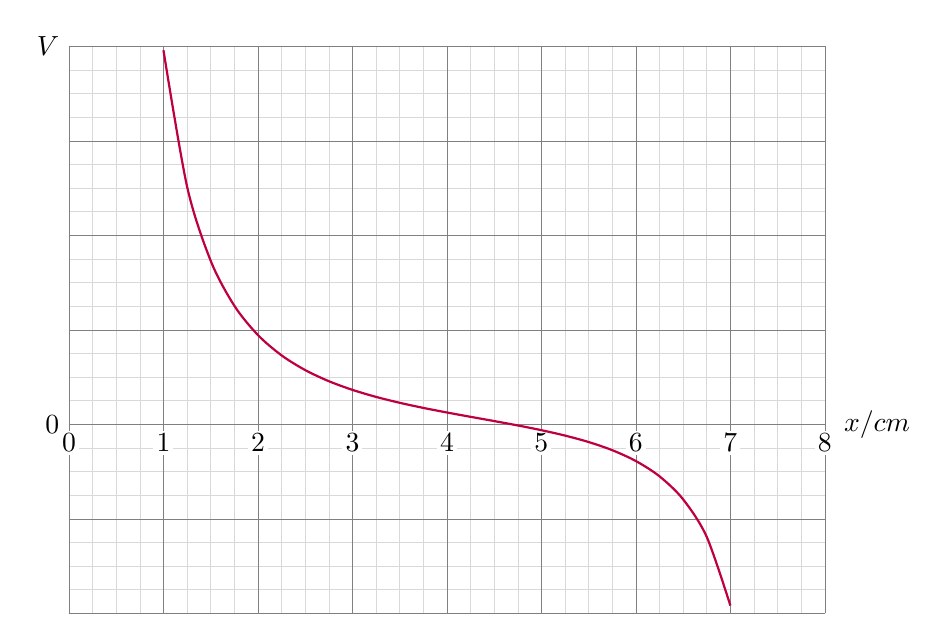
\begin{tikzpicture}[scale=1.2]
	\draw[style=help lines,step=0.25,gray!30] (0,-2) grid (8,4);
	\draw[style=help lines,step=1] (0,-2) grid (8,4);
	\node[left] at (0,4) {$V$};
	\node[left] at (0,0) {0};
	\foreach \x in {0,1,...,8} {
		\draw[white,fill] (\x-0.1,-0.32) rectangle (\x+0.1,-0.08);
		\node[below] at (\x,0) {$\x$};
	}
	\draw[thick, purple, domain=1:7, samples=25, smooth, variable=\x] plot (\x,{4/\x/\x-2/(8-\x)/(8-\x)});
	\node[right] at (8.1,0) {$x/\text{cm}$};
	\end{tikzpicture}
\end{figure}

\sol greatest force means greatest field strength, which means maximum potential gradient 

largest gradient of $V$-$x$ curve at $x=1$ cm, so greatest force at $x=1$ cm \eoe

\example{electric field due to an isolated point charge}

we have learned that the electric potential due to a point charge is: $V = \frac{Q}{\ec r}$
	
using $E = -\frac{\dd V}{\dd r}$, we have $E = -\frac{\dd}{\dd r}\left( \frac{Q}{4\pi\epsilon_0r} \right) = -\frac{Q}{4\pi\epsilon_0}\frac{\dd}{\dd r}\left(\frac{1}{r}\right) = \frac{Q}{4\pi\epsilon_0r^2}$

this agrees with the expression for field strength due to an isolated charge \eoe

\question{For the electric field due to a charged metal sphere (see Example \ref{ex-metal-sphere}), convince yourself that the field strength equals negative gradient of potential at any point.}

\question{We have seen the statement field strength equals negative potential gradient holds for electric fields. Does it also hold for gravitational fields?}




\subsubsection*{uniform fields revisited}

given two oppositely-charged metal plates separated by a distance of $d$

if p.d. between the plates is $V$, then electric field strength between is given by $E = \frac{V}{d}$\footnote{You should have learned this in AS-level physics.}

we will derive this result using the theorem introduced in the last section

\begin{figure}[ht]
\centering
\begin{minipage}{0.48\textwidth}
	\centering
	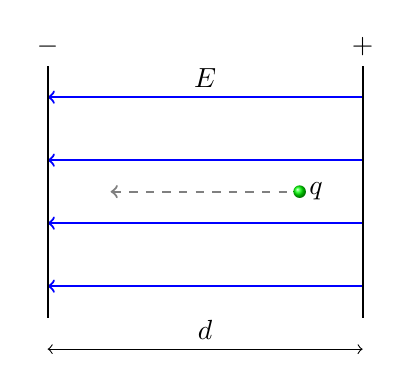
\begin{tikzpicture}[scale=0.8]
	\foreach \s in {1,2,3,4}
	\draw[thick,blue,<-] (0,\s) -- (5,\s);
	\draw (2.5,4) node[above]{$E$};
	\draw [thick,gray,dashed,<-] (1,2.5) -- (4,2.5);
	\shade [ball color = green] (4,2.5) circle [radius=0.1] node[right]{$q$};
	\draw [thick] (5,0.5) -- (5,4.5) node[above]{$+$};
	\draw [thick] (0,0.5) -- (0,4.5) node[above]{$-$};
	\draw[<->] (0,0) -- (5,0) node[midway, above] {$d$};
	\end{tikzpicture}
\end{minipage}\hfil
\begin{minipage}{0.48\textwidth}
	\centering
	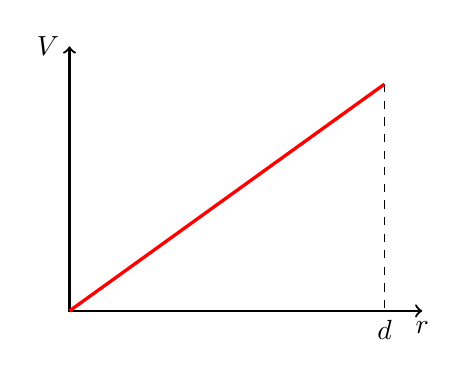
\begin{tikzpicture}[scale=0.8]
		\draw [thick,<->] (0,4.2) node[left]{$V$} -- (0,0) -- (5.6,0) node[below]{$r$};
		\draw[dashed] (5,3.6) -- (5,0) node[below]{$d$}; 
		\draw [very thick,red] (0,0) -- (5,3.6);
	\end{tikzpicture}
\end{minipage}
\captionsetup{labelformat=empty}

\caption{moving a test charge in a uniform electric field}
\end{figure}


moving a test charge $q$ in a uniform field, work done by electric force: $W=Fd = Eqd$
		
change in P.E.: $\Delta E_p = -W = -Eqd$

change in potential: $\Delta V = \frac{\Delta E_p}{q} = - Ed$, or $E=-\frac{\Delta V}{d}$

plotting $V$-$r$ graph, $\text{gradient of line}=-E$

the minus sign means field strength points in the direction such that potential decreases

i.e., electric field acts from high potential to low potential



\subsubsection*{electric field due to two positive point charges}

two point charges $+Q_1$, $+Q_2$ are separated by a distance of $D$

let's look into the electric field along the segment joining the two charges 

\begin{center}
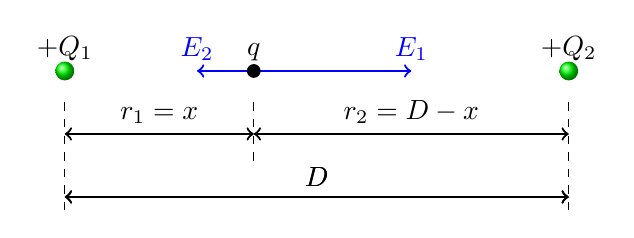
\begin{tikzpicture}[scale=0.8]
\shade [ball color = green] (-4,0) node[above]{$+Q_1$} circle (0.15);
\shade [ball color = green] (4,0) node[above]{$+Q_2$} circle (0.15);
\draw [thick, <->] (-4,-2)--(4,-2) node[midway,above]{$D$} ;
\draw [thick, <->] (-4,-1)--(-1,-1) node[midway,above]{$r_1=x$};
\draw [thick, <->] (-1,-1)--(4,-1) node[midway,above]{$r_2=D-x$};
\draw [thick, <->] (-4,-2)--(4,-2) node[midway,above]{$D$} ;
\draw [dashed] (-4,-0.5) -- (-4,-2.2);
\draw [dashed] (4,-0.5) -- (4,-2.2);
\draw [dashed] (-1,-0.5) -- (-1,-1.5);
\draw [->,thick,blue] (-1,0) -- ++(-0.9,0) node[above]{$E_2$};
\draw [->,thick,blue] (-1,0) -- ++(2.5,0) node[above]{$E_1$};
\draw [fill] (-1,0) node[above]{$q$} circle [radius=0.1];
\end{tikzpicture}
\end{center}

combined potential: $V = V_1 + V_2 = \frac{Q_1}{4\pi\epsilon_0r_1} + \frac{Q_2}{4\pi\epsilon_0r_2} = \frac{1}{4\pi\epsilon_0}\left(\frac{Q_1}{x} + \frac{Q_2}{D-x}\right)$

combined field strength: $E = E_1 - E_2 = \frac{Q_1}{4\pi\epsilon_0r_1^2} - \frac{Q_2}{4\pi\epsilon_0r_2^2} = \frac{1}{4\pi\epsilon_0}\left(\frac{Q_1}{x^2} - \frac{Q_2}{(D-x)^2}\right)$

notice that when computing $V$, we carry out \emph{scalar sum}

but for $E$, we carry out \emph{vector sum}, i.e., directions of $E_1$ and $E_2$ become important

$V$-$x$ graph and $E$-$x$ graph for the case where $Q_1=3Q_2$ are sketched

\begin{center}
	\begin{tikzpicture}[scale=1.35]
	\draw[thick,->] (0,-2) -- (0,4.8);
	\draw[thick,->] (0,0) -- (9,0) node[below]{$x$};
	\draw [thick,color=blue,domain=0.3:7.7,samples=60,smooth,variable=\x] plot (\x,{(.24/\x/\x-.08/(8-\x)/(8-\x))*1.5}) node[below]{$E$};
	\draw [thick,color=red,domain=0.3:7.7,samples=60,smooth,variable=\x] plot (\x,{(.3*3/\x+.1*3/(8-\x))*1.5}) node[above]{$V$};
	\draw[dashed] (8,-2) -- (8,3);
	\shade [ball color = green] (0,0) node[below right]{$+Q_1$} circle (0.15);
	\shade [ball color = green] (8,0) node[below right]{$+Q_2$} circle (0.15);
	\end{tikzpicture}
\end{center}

\question{Convince yourself that field strength is indeed given by negative potential gradient. You may interpret it either graphically (think about gradient of tangent along the curve) or algebraically (think about the derivative of $V$).}

\question{We have looked into the electric field between two positively-charged particles. Discuss the cases where (a) both particles are negatively charged, (b) the two particles carry opposite charges.}